\documentclass[letterpaper]{article}
\usepackage{iccc}

\usepackage{times}
\usepackage{helvet}
\usepackage{courier}
\usepackage{graphicx}
\usepackage[titlenotnumbered, boxruled]{algorithm2e}
\usepackage{amsmath}
\usepackage[T1]{fontenc}
\usepackage{hyperref}

\pdfinfo{
/Title (Automatic Puzzle Level Generation: A General Approach using a Description Language)
/Subject (Proceedings of CCGW 2015)
/Author (Ahmed Khlifa, Magda Fayek)}
% The file iccc.sty is the style file for ICCC proceedings.
%
\title{Automatic Puzzle Level Generation:\\
A General Approach using a Description Language}
\author{Ahmed Khalifa \and Magda Fayek\\
Computer Engineering Department\\
Faculty of Engineering, Cairo University\\
Cairo University Road, Giza, Egypt\\
amidos2002@hotmail.com, magdafayek@ieee.org\\
}
\setcounter{secnumdepth}{0}

\newcommand{\chref}[1]{Chapter~\ref{Chapter:#1}}
\newcommand{\appref}[1]{Appendix~\ref{Appendix:#1}}
\newcommand{\secref}[1]{Section~\ref{Section:#1}}
\newcommand{\eqnref}[1]{Equation~\ref{Equation:#1}}
\newcommand{\tabref}[1]{Table~\ref{Table:#1}}
\newcommand{\figref}[1]{Figure~\ref{Figure:#1}}
\newcommand{\algref}[1]{Algorithm~\ref{Algorithm:#1}}

\begin{document} 
\maketitle
\begin{abstract}
\begin{quote}
In this paper, we present a general technique to evaluate and generate puzzle levels made by \emph{Puzzle Script}, a videogame description language for scripting puzzle games, which was created by Stephen Lavelle\cite{puzzleScript}. In this work, we propose a system to help in generating levels for Puzzle Script. Levels are generated without any restriction on the rules. Two different approaches are used with a trade off between speed (Constructive approach) and playability (Genetic approach). These two approaches use a level evaluator that calculates the scores of the generated levels based on their playability and challenge. The generated levels are assessed by human players statistically, and the results show that the constructive approach is capable of generating playable levels up to 90\%, while genetic approach can reach up to 100\%. The results also show a high correlation between the system scores and the human scores.
\end{quote}
\end{abstract}

\section{Introduction}
During the early days of Video Games, games were created by few people in their spare time. Most of the time was spent in programming the game, while a small portion was dedicated for graphics, sounds, and music because of the technical limitations of the devices at that time. As these limitation are no more, producing a game takes more time than before. Most of that time is spent on creating content for the game (graphics, music, sounds, levels, and ...etc)\cite{budgetAAA}; for example creating graphics for a huge main stream game may take hundreds of artist working for a year or two. That is why the production cost of a huge game reaches millions of dollars\cite{gameCost}.\\\par

That huge production cost is one of the reasons for the use of Procedural Content Generation(PCG). PCG means generating game content using a computer. It was first developed due to technical limitations (small disk space) and the need to provide a huge amount of content\cite{pcgFirstGame}. Although technical difficulties become history and storage is no longer a problem, PCG is still one of the hot topics in Video Games Industry and Research. PCG helps us reduce development time and cost, be creative, and understand the process of creating game content. PCG can be used to generate different game aspects for example Textures, Sounds, Music, Levels, Rules, and ...etc.\\\par

Level Generation has been in industry since dawn of games in order to decrease the game size, but it is now used to introduce huge amount of levels that humans can not generate manually in reasonable time. Level Generation has always been done for a specific game using lots of hacks to improve the output result. These hacks cause the output levels to follow certain guidelines which may cause elimination of huge amounts of possible levels but on the other hand these guidelines ensure that the output levels are all playable (can reach goal of the game) and satisfactory by all players\cite{mcGenerateEverything}.\\\par

In this paper, we propose a system to generate playable puzzle levels without any restrictions or hacks. we utilize small prior knowledge about puzzle script to ensure playability and challenge.

\section{Background}
We can not generate general levels without having a methodology to describe the games. Video Game Description Language(VGDL) was originally invented to help on the work for General Video Game Playing(GVGP)\cite{gvgp} at Standford University. Puzzle Script(PS) is a VGDL created by Stephan Lavelle to help game designers and developers to create puzzle games\cite{puzzleScript}. Games generated by PS are time stepped games similar to Sokoban\cite{sokoban}. PS file starts with some meta data like game name, author name, and website then it is divided into 7 sections objects, legend, sounds, collision layers, rules, win conditions, and levels. In this work, we focus on rules, win conditions, and levels section. Rules are a set of production rules that govern how the game will be played. For example, \emph{[> Player | Crate] -> [> Player | > Crate]} means if there is a Player and Crate beside each other, and the Player moves towards the Crate, then both the Player and the Crate will move in the same direction. Win conditions are group of rules that identify when the level should end. Levels are 2D matrices showing the current configuration for each game level using objects identified in objects section.

\section{Literature Review}
As there is nothing before like this work, this section will show all previous work that can be slightly related to our problem. One of the earliest research in Puzzle Games was by Murase et al.\cite{sokobanLevelGenerationOld}. Murase et al. work focused on generating well designed solvable levels for Sokoban\cite{sokoban}. Their work consists of 3 stages:
\begin{itemize}
	\item \emph{Generate:} Responsible for generating Level Layouts. Level Layouts is generated by placing predefined templates at random positions. Goal locations and crates are placed afterwards at random positions such that each goal location is reachable from the player location and each crate is reachable from a unique goal location.
	\item \emph{Check:} Responsible for checking for playability. The system uses Breadth First Search (BFS) to check for solution. All unsolvable levels are removed in this step.
	\item \emph{Evaluate:} Responsible for selecting best generated levels. The system removes all levels that have a solution that is very short, contains less than four direction changes, or does not contain any detours.
\end{itemize}
Results show that for every 500 generated levels only 14 are considered as good levels. These good levels are characterized by having a short solution sequence due to the usage of BFS.\\\par

Taylor and Parberry\cite{sokobanLevelGenerationNew} followed Yoshio Murase et al.\cite{sokobanLevelGenerationOld} work to improve generated level quality. Their system consists of 4 stages:
\begin{itemize}
	\item \emph{Generating empty room:} Responsible in generating Level Layouts like Yoshio Murase et al.\cite{sokobanLevelGenerationOld} work. After generating the layouts, the system discards any level that is not completely connected, has huge empty space, or has number of empty floors less than the planned number of boxes and goals.
	\item \emph{Placing goals:} Responsible for finding best suitable goal locations. The system use a brute force algorithm to try every possible combination for goal locations.
	\item \emph{Finding the farthest state:} Responsible for placing crates at farthest location from its goal location. This process is done using a similar algorithm to BFS. The algorithm expands all the reachable locations from a goal location and returns the farthest location. The farthest location is calculated using a box line metric heuristic which calculates the number of unrepeated moves required to reach that location.
	\item \emph{Evaluating generated levels:} Responsible for evaluating the generated levels. Evaluation is done using some heuristic functions. For example: number of box pushes in the solution, number of levels found at same solution depth, number of box lines, number of boxes, and ...etc.  
\end{itemize}
The generated levels are not suffering from the problem of short level sequences presented in Yoshio Murase et al.\cite{sokobanLevelGenerationOld} work. As the target number of crates increases, the generation process takes more time but delivers much more interesting and difficult levels.\\\par

Rychnovsky\cite{fruitDatingPCG} work focused on generating levels for his new game Fruit Dating\cite{fruitDating}. Rychnovsky developed a level editor that can be used to generate new levels or test playability of certain level. Generating new levels is done using the following steps: 
\begin{itemize}
	\item \emph{Generating level structure:} The system generates level structures based on 2 steps. First step is generating external walls. External walls are generated at any random location connected to the border with short random length. Second step is generating inner walls. Inner walls are generated at any free location with free 3x3 locations.
	\item \emph{Placing game objects:} The system generates fruits at random locations based on predefined weights. Every empty location is assigned a score using these weights. Locations with highest scores are selected. Other game objects use the same strategy but using different weights.
	\item \emph{Checking for a solution:} The system use an algorithm similar to BFS to find the solution of the generated level. If no solution found, the level is discarded.
\end{itemize}
The technique doesn't take more than couple of minutes to generate a level. The main problem is there is no way to influence difficulty in the generated levels.\\\par

Shaker et al.\cite{ctrAutomaticGeneration} worked on generating levels for physics based puzzle games. They applied their technique on Cut The Rope(CTR)\cite{cutTheRope}. Shaker et al. used Grammar Evolution (GE) technique to generate levels for CTR. GE is a result of combining an evolutionary algorithm like GA with a grammar representation. The grammar is designed to ensure that every game object appears at least one time. The fitness function used to rate the generated levels depends on some heuristic measures based on prior knowledge about the game. For example: Candy should be placed higher than the OmNom, OmNom must be placed below the lowest rope, and ...etc. Since using heuristics does not ensure playability, each generated level is played 10 time using a random player. The fitness score is reduced by a large number if no solution was found. Shaker et al. generated 100 playable levels and analyzed them according to some metrics such as frequency, density, and ...etc.\\\par

Shaker et al.\cite{ctrSimulationApproach} conducted their research on CTR to improve generated level quality. They replaced the random player with an intelligent one. Two types of automated players are developed. The first one takes an action based on the current properties of all objects in the level. While the second one takes an action based on the reachability between every level objects and the candy at every time step based on the candy's current position, velocity, and direction. The generated levels are far more diverse because the random player discards some potential levels in the search space.\\\par

Shaker et al.\cite{ctrProgressiveApproach} introduced a new generation technique named Progressive Approach. Progressive Approach can be used on any kind of games to reduce the generation time. Progressive Approach is divided into two main steps:
\begin{itemize}
	\item \emph{Time-line Generation:} GE is used to evolve a time-line of game events.
	\item \emph{Time-line Simulation:} Evolved time-lines are simulated using an intelligent agent. The agent utilize prior knowledge about the game to map the time-line to a possible level layout. Based on the agent result and some desirable heuristics, each time-line is assigned a fitness score.
\end{itemize}
Shaker et al. tested the new technique on CTR and compared its results with their previous work\cite{ctrSimulationApproach}. The results indicates a huge decrease in generation time, as it changed from 82 seconds towards 9.79 seconds. Although Progressive Approach is much faster and better from previous, it is difficult to determine the level difficulty before simulation. Also the quality of the levels depends on the intelligent agent used in the mapping process.\\\par

Williams-King et al.\cite{kgrAutomaticGeneration} work focused on generating levels for their game KGoldRunner. KGoldRunner is just a port for the famous game Lode Runner\cite{lodeRunner}.Williams-King et al. used GA to generate random levels. Generated levels are evaluated using fitness function based on some prior knowledge about the game. For example: checking level connectivity using BFS between starting point and all gold coins. High score levels are simulated using an automated player that tries to collect all gold chunks using 20 different paths. The number of solvable paths indicates the level difficulty. As the number of generations increase more time is required but more levels are likely to be solvable.\\\par

Smith et al.\cite{refractionStudy} worked on generating puzzle levels for Refraction\cite{refraction}. Smith et al. divided his generator into 3 main components: 
\begin{itemize}
	\item \emph{Mission Generation:} Responsible for generating a general outline showing level solutions. 
	\item \emph{Level Embedder:} Responsible for translating the general outline to a geometric layout.
	\item \emph{Puzzle Solver:} Responsible for testing generated level for solution.
\end{itemize} 
These components are implemented into two different ways (Algorithmic approach and Answer Set Programming (ASP)). Results shows that ASP is faster than Algorithmic approach specially in Puzzle Solver module, while Algorithmic approach produces more diverse levels than ASP.

\section{Methodology}
Level Generation is not an easy task specially when the game rules are not known before generation. Most of the previous work in the Puzzle Level Generation (refer to \chref{Chapter3}) was limited for generating levels for a specific game. Although some research suggested a general technique to generate levels, it is still based on designing a game specific fitness function. In this work, we suggest some global metrics for Puzzle Games that can help in generating levels with the minimum prior knowledge.\\\par

Our approach relies heavily on the understanding of the current game rules and some prior knowledge about Puzzle Script language. \figref{levelGenBlockDiagram} shows a high level block diagram of the system. The following subsections will describe each block in details.

\begin{figure}[ht]
  	\centering
    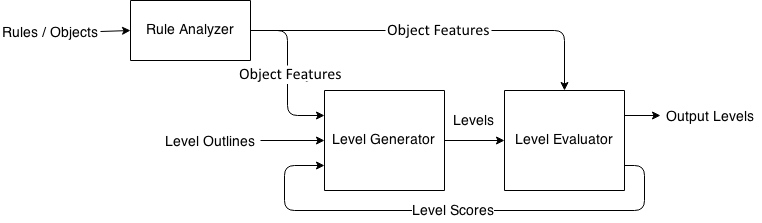
\includegraphics[width=0.45\textwidth]{Images/levelGenBlockDiagram}
    \label{Figure:levelGenBlockDiagram}
    \caption{High level system block diagram for Level Generation}
\end{figure}

The system starts by analyzing the current game rules using a Rule Analyzer. The Rule Analyzer utilizes some basic information about Puzzle Script rules to understand the importance of each game object and its basic functionality.\\\par

The output of the Rule Analyzer (Rule Analysis) and the Level Outlines are fed to a Level Generator. The Level Generator is responsible for generating initial level layouts. It utilizes the Rule Analysis to insert game objects at suitable positions in the Level Outlines. Level Generator uses two different approaches: a Constructive Approach and a Genetic Approach. The Constructive Approach is faster in generation but produce less diverse levels, while Genetic Approach requires more time but give access to a vast majority of levels.\\\par

The generated levels are subjected to a Level Evaluator. The Level Evaluator uses an automated player to play the generated levels. Based on the result of each play, the Level Evaluator gives a score for the level based on some heuristic measures. These measures make sure the resulting level is playable and not trivial.\\\par

In case of the Constructive Approach, the system selects the best scored levels to output them, while the Genetic Approach enhances the output levels using GA.

\subsection{Rule Analyzer}\label{Section:ruleAnalyzer}
The Rule Analyzer is the first module in our system. It analyzes game rules and extract some useful information about each object. The extracted information is fed to the Level Generator and the Level Evaluator. Each object is assigned:
\begin{itemize}
	\item \emph{Type:} Object type depends on its presence in the Puzzle Script file. There are 4 different types:
	\begin{itemize}
		\item \emph{Rule Object:} Any object that appears in a rule is defined as a rule object. Rule objects are essential for rules to be applied.
		\item \emph{Player Object:} It is defined by name "Player" in the Puzzle Script. It is the main game entity. It can move freely without any restriction. Any level must have at least 1 player object. Player object is a Rule Object as well.
		\item \emph{Winning Object:} They are objects appearing in the winning condition. At least one of them is a Rule Object or a Player Object.
		\item \emph{Solid Object:} All objects that does not appear in any rule but on the same collision layer with a Rule Object.
	\end{itemize}
	\item \emph{Subtype:} each Rule Object is assigned a Subtype based on its presence in game rules. These subtypes are:
	\begin{itemize}
		\item \emph{Critical Object:} is an object that has appeared with the Player object and one of the Winning Objects in the rules.
		\item \emph{Normal Object:} same like the Critical Object but it only appears with one of them.
		\item \emph{Useless Object:} is an object that neither appears with the Player Object nor the Winning Objects in any rule.
	\end{itemize}
	\item \emph{Priority:} It reflects the number of times each object appears in the rules.
	\item \emph{Behaviors:} Behaviors are analyzed from the difference between the left hand side and the right hand side of each rule for every object. Every object can have one or more behavior. There are 4 kinds of behaviors:
		\begin{itemize}
			\item \emph{Move:} If an object on the left hand side have different movement than the right hand side, this object has a Move behavior. For example, In the following rule Crate moves when Player approaches it.
			\begin{center}
				[ > Player | Crate ] -> [ > Player | > Crate ]
			\end{center}
			\item \emph{Teleport:} An object is considered to have a Teleport behavior if its location in the rule changes from the left hand side to the right hand side. For example, In the following rule Crate changes position with Player on collision.
			\begin{center}
				[ > Player | Crate ] -> [ Crate | Player ]
			\end{center}
			\item \emph{Create:} If the number of a certain object on the left hand side is less than its number on the right hand side, then this object has a Create behavior. For example, In the following rule, Crate is created when Player moves to an empty place.
			\begin{center}
				[ > Player | \ \ \ \ ] -> [ Crate | Player ]
			\end{center}
			\item \emph{Destroy:} If the number of a certain object on the left hand side is greater than its number on the left hand side, then this object has a Destroy behavior. For example, In the following rule, the three Crates are destroyed when they are aligned beside each other.
			\begin{center}
				[ Crate | Crate | Crate ] -> [ \ \ \ \ | \ \ \ \ | \ \ \ \ ]
			\end{center}
		\end{itemize}
	\item \emph{Minimum Number:} It is the maximum number of times for an object to appear in the left hand side of game rules. For example consider the following group of rules:
	\begin{center}
		[ > Player | Crate ] -> [ > Player | > Crate ]
	\end{center}
	\begin{center}
		[ > Crate | Crate ] -> [ > Crate | > Crate ]
	\end{center}
	The Crate object appeared in the both rules. The first rule the Crate object appeared once, while the second rule it appeared twice. This means the minimum number of Crates is two. This is not the case when an object have a Create behavior. Create rules are responsible for generating objects. The Minimum Number of the Create objects is updated to reflect the least number of appearances in the Create rules. For example the following rules have two Create rules (the first and the third).
	\begin{center}
		[ > Player | \ \ \ \ ] -> [ Crate | Player ]
	\end{center}
	\begin{center}
		[ > Crate | Crate ] -> [ > Crate | > Crate ]
	\end{center}
	\begin{center}
		[ Gem | Crate | Gem ] -> [ Crate | Crate | Crate ]
	\end{center}
	The number of Crate objects in each rule are 0, 2, 1 respectively. In normal case, the minimum number of Crate object will be 2. Since Crate object have Create behavior (in both the first and the third rule) then the minimum number of objects will be zero instead.
	\item \emph{Relations:} It is a list of all objects that appears in the same rule with a certain object. For example, In the following rules, Crate has relations with Player and Lava, Player has a relation with Crate, and Lava has a relation with Crate.
	\begin{center}
		[ > Player | Crate ] -> [ > Player | > Crate ]
	\end{center}
	\begin{center}
		[ > Crate | Lava ] -> [ \ \ \ \ | \ \ \ \ ]
	\end{center}
	Each object has a special list for the left hand side only beside the main Relations list.	
\end{itemize}

\subsection{Level Generator}
The Level Generator is responsible for creating a level in the best possible way. Two approaches were used to generate levels. The following subsections will discuss each one of them.

\subsubsection{Constructive Approach}\label{Section:constructiveApproach}
Constructive Approach uses information from the Rule Analyzer to modify the Level Outlines. In this approach, several levels are generated using a certain algorithm and the best levels are selected. A pseudo code for the algorithm is presented in \algref{constructiveApproach}.\\

\begin{algorithm}[ht]
	\KwData{level outline, rule analysis}
	\KwResult{modified level outline}
	\BlankLine
	numberObjects = Get the number of objects for each object type\;
	\BlankLine
	levelOutline = Insert Solid Objects in the level outline\;
	levelOutline = Insert Winning Objects in the level outline\;
	levelOutline = Insert Player Object in the level outline\;
	levelOutline = Insert Critical Objects in the level outline\;
	levelOutline = Insert Rule Objects in the level outline\;
	\BlankLine
	\textbf{return} levelOutline\;
	\caption{Pseudo algorithm for the Constructive Approach}
	\label{Algorithm:constructiveApproach}
\end{algorithm}
The algorithm consists of two main part. The first part is responsible for determining the amount of objects that should be presented in the current level outline. The second part is responsible for inserting game objects in an intelligent way to the current level outline. The order of the insertion algorithm places the most important game objects first to ensure playability.\\\par

\algref{numberObjects} shows the process of calculating the amount of objects. The algorithm starts by determining the percentages for each object type. Each object type contributes by a percentage equal to its minimum number to make sure that all rules can happen. A cover percentage is calculated based on the number of critical and winning objects. The value of the cover percentage is inversely proportional with the summation of both critical and winning objects. Critical and Winning Objects are the main game objects, without them game may not be playable at all. The increase in their numbers causes the level to be more difficult and more complex. Having a small cover percentage when they are huge, makes sure the game is not very complex.\\

\begin{algorithm}[ht]
	\KwData{level outline, rule analysis}
	\KwResult{Number of Objects for each type}
	\BlankLine
	percentages[Winning Object] = Minimum Number[Winning Object 1] + Minimum Number[Winning Object 2]\;
	\If{Player Object is a Winning Object}{
		percentages[Winning Object] = 2\;
	}
	percentages[Solid Object] = Number of different kinds of Solid Objects\;
	percentages[Critical Object] = Summation of the minimum number of all Critical Objects\;
	percentages[Rule Object] = Summation of the minimum number of all Rule Objects\;
	Divide all percentages by their total summation\;
	\BlankLine
	coverPercentage = 1 - percentages[Winning Object] - percentages[Critical Object]\;
	totalNumber = coverPercentage * total free area in the level outline\;
	numberObjects = totalNumber * weights * percentages\;
	numberObjects[Player] = 1\;
	\BlankLine
	\textbf{return} numberObjects\;
	\caption{Get the number of objects algorithm}
	\label{Algorithm:numberObjects}
\end{algorithm}

The following algorithms are responsible for inserting objects based on the numbers resulted from the previous part. Most of them always need to find the most suitable empty locations to insert the new Object. The most suitable location is calculated based on the features of the inserted object. If the object has a Move behavior, it should be inserted at spots with the most free locations around it. Otherwise any random free location is okay.\\\par

\algref{solidObjects} shows the insertion algorithm for Solid Objects. The algorithm inserts a random solid objects at a random empty space (as Solid Object has not a Move behavior) in the level outline. The algorithm is repeated for several times based on its number. The same idea is used for inserting Player Object in \algref{playerObject} but for only one time.\\

\begin{algorithm}[ht]
	\KwData{level outline, rule analysis, number of objects}
	\KwResult{modified level outlines}
	\BlankLine
	\While{numberObjects[Solid Object] > 0}{
		object = Get a random solid object\;
		location = Get a suitable empty location\;
		levelOutline[location] = object\;
		numberObjects[Solid Object] -= 1\;
	}
	\BlankLine
	\textbf{return} levelOutline\;
	\caption{Solid Objects Insertion Algorithm}
	\label{Algorithm:solidObjects}
\end{algorithm}

Before inserting the Player to the level, Winning Objects should be inserted. \algref{winningObjects} is responsible for inserting Winning Objects into the level outline. The algorithm generates an equal amount of both winning objects except if any of these objects have a Create behavior. The amount of the generated Winning Objects must be a multiple of their minimum number to ensure that all rules can be applied. The first winning object is inserted at any suitable empty location, while the other must be inserted at the farthest suitable empty location. Inserting at a very far location ensures a more difficult level. If the Winning Rule is No then the second object will be inserted at the same location of the first object.\\

\begin{algorithm}[ht]
	\KwData{level outline, rule analysis, number of objects}
	\KwResult{modified level outlines}
	\BlankLine
	\eIf{Winning Objects have Create beahvior}{
		minObject1 = Minimum Number(Winning Object 1)\;
		minObject2 = Minimum Number(Winning Object 2)\;
	}{
		minObject1 = Max(Minimum Number(Winning Object 1), Minimum Number(Winning Object 2))\;
		minObject2 = minObject1\;
	}
	\BlankLine
	\While{numberObjects[Winning Object] > 0}{
		\For{1 \KwTo minObject1}{
			location = Get a suitable empty location for Winning Object 1\;
			levelOutline[location] = Winning Object 1\;
			numberObjects[Winning Object] -= 1\;
		}
		
		\BlankLine
		\For{1 \KwTo minObject2}{
			\If{Winning Rule != No}{
				location = Get the farthest suitable empty location for Winning Object 2\;
			}
			levelOutline[location] = Winning Object 2\;
			numberObjects[Winning Object] -= 1\;
		}
	}
	\BlankLine
	\textbf{return} levelOutline\;
	\caption{Winning Objects Insertion Algorithm}
	\label{Algorithm:winningObjects}
\end{algorithm}

\begin{algorithm}[ht]
	\KwData{level outline, rule analysis, number of objects}
	\KwResult{modified level outlines}
	\BlankLine
	location = Get a suitable empty location for the Player Object\;
	levelOutline[loction] = Player Object\;
	\BlankLine
	\textbf{return} levelOutline\;
	\caption{Player Object Insertion Algorithm}
	\label{Algorithm:playerObject}
\end{algorithm}

\algref{criticalObjects} is responsible for inserting Critical Objects. Critical Objects are one of the most important objects in the game. As they are connected with both Player and Winning Objects. In some games, levels are not solvable without Critical Objects. For example, the following rules are from game called DestroyGame. The game goal is to destroy all Gem objects. Gem objects can be destroyed if they are aligned with 2 Crate objects. Crate objects can be pushed by the Player object.
\begin{center} [ > Player | Crate ] -> [ > Player | > Crate ]\end{center}
\begin{center} [ Crate | Gem | Crate ] -> [ \ \ \ \ | \ \ \ \ | \ \ \ \ ]\end{center}
From these rules Crate is a critical object as it is connected with Gem and Player objects. If there is no Crates in the level, the game will be unplayable. For that reason the algorithm ensures inserting the minimum Number of all the critical objects. The algorithm adds more critical objects according to its number. Each critical object has a chance to appear directly proportional with its Priority feature.\\

\begin{algorithm}[ht]
	\KwData{level outline, rule analysis, number of objects}
	\KwResult{modified level outlines}
	\BlankLine
	\ForEach{object in Critical Objects}{
		\For{1 \KwTo Minimum Number of object}{
			location = Get a suitable empty location\;
			levelOutline[location] = object\;
			numberObjects[Critical Object] -= 1\;
		}
	}
	\BlankLine
	\While{numberObjects[Critical Object] > 0]}{
		object = Choose a random Critical Object based on its priority\;
		\For{1 \KwTo Minimum Number of object}{
			location = Get a suitable empty location\;
			levelOutline[location] = object\;
			numberObjects[Critical Object] -= 1\;
		}
	}
	\BlankLine
	\textbf{return} levelOutline\;
	\caption{Critical Objects Insertion Algorithm}
	\label{Algorithm:criticalObjects}
\end{algorithm}

Same is done with Rule Objects in \algref{ruleObjects}. Random Rule Objects are inserted to the map based on their Priority feature.\\

\begin{algorithm}[ht]
	\KwData{level outline, rule analysis, number of objects}
	\KwResult{modified level outlines}
	\BlankLine
	\While{numberObjects[Rule Object > 0]}{
		object = Choose a random Rule Object based on its priority\;
		\For{1 \KwTo Minimum Number of object}{
			location = Get a suitable empty location\;
			levelOutline[location] = object\;
			numberObjects[Critical Object] -= 1\;
		}
	}
	\BlankLine
	\textbf{return} levelOutline\;
	\caption{Rule Objects Insertion Algorithm}
	\label{Algorithm:ruleObjects}
\end{algorithm}

\subsubsection{Genetic Approach}\label{Section:geneticApproach}
This method uses GA to evolve level outlines to playable levels. Elitism is used to ensure that the best levels are carried to the next generation.\\\\
\emph{\textbf{Chromosome Representation:}} In this technique levels are represented as 2D matrix. Each location value represents all the objects at that location.\\\\
\emph{\textbf{Genetic Operators:}} Crossover and Mutation are used to ensure better levels in the following generations. One point crossover is used where a point (x, y) is selected from the first chromosome and all previous rows (having smaller x) are swapped with the second chromosome. Mutation changes any random selected position using the following:
\begin{itemize}
	\item \emph{Creating an object:} a random object is selected to replace an empty position in the level. In "No" winning condition, the two winning objects are created at the same location.
	\item \emph{Deleting an object:} a random object from the level is deleted.
	\item \emph{Changing object position:} a random empty position is swapped with a non-empty one.
\end{itemize}
The mutation operation happens by subjecting the level outline to these 3 methods using different probabilities. The Creating and deleting an object have lower probability than the changing object position.\\\\
\emph{\textbf{Initial Population:}} Three different techniques are used to generate an initial population for the GA. These techniques are:
\begin{itemize}
	\item \emph{Random Initialization:} The population is initialized as mutated versions of the empty level outline. This technique takes very long time to find a good designed level as it search in the whole space.
	\item \emph{Constructive Initialization:} The population is initialized using the Constructive Approach algorithm. Using the algorithm tighten the search space so less time is required to find good playable levels.
	\item \emph{Mixed Approach:} The population is initialized as a mixture between the Random Initialization and the Constructive Initialization. A portion is initialized using the Constructive Approach Algorithm and some mutated versions, while the other portion is the same like the Random Initialization. Using that algorithm ensure more diversity than the previous two approaches.
\end{itemize}
More details about the results of each algorithm will be discussed in \chref{Chapter5}.

\subsection{Level Evaluator}\label{Section:levelEvaluator}
Level Evaluator is responsible for evaluating the generated levels. Level evaluation is based on some global knowledge about the Puzzle Script Language and Puzzle Games. The easy way to evaluate a puzzle level is to measure its level playability. Level playability is achieved by using an automated player which will be discussed later. Playability is not enough to judge puzzle levels. Some other metrics must be used to ensure that the solution have more moves with some thinking ahead. \figref{diffLevelsSokoban} shows several levels designed for Sokoban game where all are playable but some of them are more interesting than the others. The first level is a very easy level which can be solved in one move. The second level need more moves which is more interesting, but it has a straight forward solution. The last level is not an easy to solve, it needs some prior thinking which is more interesting than the previous two.

\begin{figure}[ht]
  	\centering
    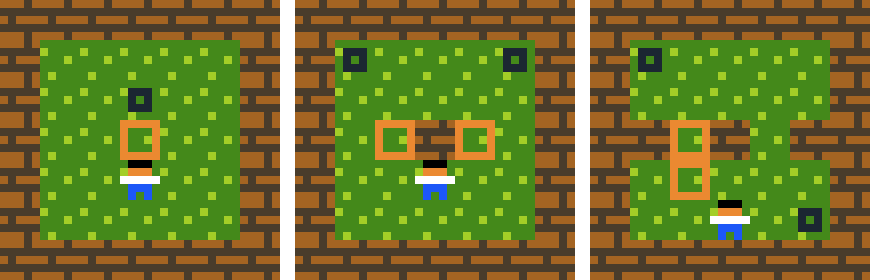
\includegraphics[width=0.45\textwidth]{Images/diffLevelsSokoban}
    \label{Figure:diffLevelsSokoban}
    \caption{Examples on different levels for Sokoban game}
\end{figure}

The example shows the need for using heuristic measures to ensure more interesting levels.

\subsubsection{Automated Player}\label{Section:automatedPlayer}
Our Level Evaluator uses a modified version of the BestFS Algorithm as the automated player. BestFS Algorithm was introduced in Lim et al.\cite{puzzleScriptGeneration} work. BestFS is similar to BFS algorithm but instead of exploring states sequentially, it sorts them according to a score generated from a fitness function. This causes the algorithm to explore the more important nodes first, helping it to reach the solution faster. As explained in \chref{Chapter3}, Lim et al. algorithm uses two metrics (as a fitness function) to evaluate each game state:
\begin{itemize}
	\item \emph{Distance between winning objects:} BestFS tries to either increase or decrease the distance between the winning objects according to the winning condition. The "No" rule is the only rule that need to increase the distance, while the others need to decrease it. The left image in \figref{bestFS} shows an example from Sokoban, where the distance between crates and targets is highlighted.
	\item \emph{Distance between player and winning objects:} BestFS always tries to minimize the distance between the player and the winning objects. To achieve the first metric, the player should come near the winning objects. The right image in \figref{bestFS} shows the same level from Sokoban, where the distance between player and winning objects (crates and targets) is highlighted.
\end{itemize}

\begin{figure}[ht]
	\centering
	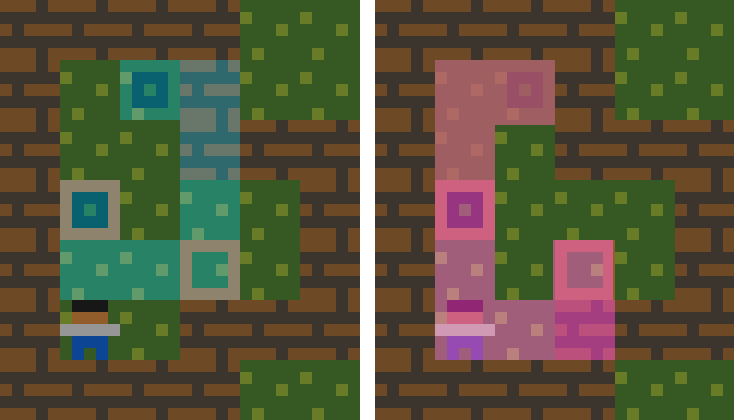
\includegraphics[width=0.45\textwidth]{Images/scoreBestFS}
	\caption{Example of distance between winning objects metric and distance between player and winning objects metric}
	\label{Figure:bestFS}
\end{figure}

These metrics works fine for all games where player is not one of the winning objects. When the player is one of the winning objects, the two metrics behaves in the same way. The player always try to move towards the winning objects regardless of any other game objects. For example, \figref{lavaGame} shows a level from a game called LavaGame. LavaGame is a puzzle game where the goal is to make the player reaches the exit. The path towards the exit is usually stuck by lava which can be destroyed by pushing a crate over it. According to the Lim et al. metrics, the player will try to move nearer to the exit by going left. This movement will not help the player to reach the exit, so the player will start wandering aimlessly trying to stumble across a movement sequence that can solve the level.

\begin{figure}
  	\centering
    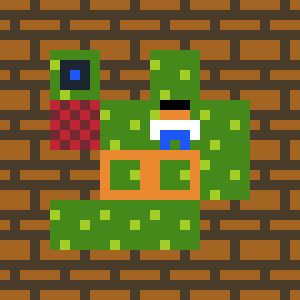
\includegraphics[width=0.3\textwidth]{Images/lavaGame}
    \label{Figure:lavaGame}
    \caption{Example level from LavaGame showing the problem in the old metrics}
\end{figure}

Player's aim is to move crates towards the lava to unblock his path towards the exit. This aim is somehow explained in the game rules, so by further analysis the game rules we can know which objects need to be closer. Returning to our example about LavaGame, the game rules are stated in the following order:
\begin{center}{[> Player | Crate] -> [> Player | > Crate]}\end{center}
\begin{center}{[> Crate | Lava] -> [ \ \ \ \ | \ \ \ \ ]}\end{center}
The first rule says if there is a player and crate beside each other and the player moves toward it, the crate will also move. The second rule says if there is a crate and lava beside each other and the crate moves toward it, both crate and lava will be destroyed. In any proper game, rules must be applied before achieving the winning condition. Based on that fact, the distance between objects on the left hand side of the rules must be decreased. The relation between objects in the left hand side of the rules is captured by the Rule Analyzer Relations list for each game object. This distance is used as the new heuristic measure beside the original ones. The three metrics are weighted with respect to each other and used as a new fitness function to evaluate game states. The weights are chosen by experimentation to ensure the best results.\\\par

The output of the automated player is essential in evaluating the level quality. Four different values are returned which capture the way the automated player plays the level. These four values are:
\begin{itemize}
	\item \emph{The score for the best reached state so far:} The score is calculated using the first metric (Distance between winning objects). The score value is in range between [0, 1], where 0 means there is no winning objects, while 1 means the player reached the solution.
	\item \emph{The movement sequence to reach the best state:} The automated player saves up all the movement happens to reach each state and returns the sequence that leads to the best state.
	\item \emph{The number of states explored while searching for the solutions:} The automated player saves the number of states that it explores before terminating.
	\item \emph{The number of rules that the game engine applies to reach the best state:} With each movement, some rules may apply through the game engine. This value returns the number of rules applied by the game engine to reach the best state.
\end{itemize}
The modified BestFS finds the solution faster than original one. More details will be explained in \chref{Chapter5}.\\\par

\subsubsection{Heuristic Measures}\label{Section:levelScoreEquation}
Heuristic measures are calculated using a weighted function of six attributes. The function is described as the following:
\begin{center}$F_{score} = 0.3 * P_{score} + 0.2 * L_{score} + 0.15 * N_{score} + 0.12 * B_{score} + 0.12 * R_{score} + 0.11 * E_{score}$\end{center}
where $P_{score}$ is the Playing Score, $L_{score}$ is the Solution Length Score, $N_{score}$ is the Object Number Score, $B_{score}$ is the Box Line Score, $R_{score}$ is the Applied Rule Score, and $E_{score}$ is the Exploration Score. The weights for each attribute are measured experimentally to reflect the importance of each features with respect to the others. The following points will further explain each of these scores.
\begin{itemize}
	\item \emph{Playing Score ($P_{score}$):} Playing score is used to ensure level playability. Instead of using a boolean value for playable or not. A float value is assigned for how much the player is near the solution. The first output of the automated player is used for that purpose. Making the domain more continuous (using float) helps in measuring the percentage of the level playability instead of using it as a constraint.\\\par
	
	Based on the work by Nielsen et al.\cite{gvgpPerformanceProfiles} which proved that Do Nothing player is an important measure for good designed games. A score is calculated for the initial level state using the same way. This score is subtracted from the previous score. The Playing Score can be expressed by the following equation:
	\begin{center}$ P_{score} = S_{play} - S_{nothing}$\end{center}
	where $S_{play}$ is the automated player score and $S_{nothing}$ is the Do Nothing player score.
	
	\item\emph{Solution Length Score ($L_{score}$):} \figref{diffLevelsSokoban} shows that interesting levels usually have more steps than the trivial ones. The first idea is to compare the length of the best movement sequence with a target value. This idea will not work as expected because solution length depends on the size of the level. For example, \figref{sokobanLenghtArea} shows different levels from Sokoban and their corresponding solution length. Its obvious that the seconds level have longer solution because it has bigger area.
	
	\begin{figure}
	  	\centering
	    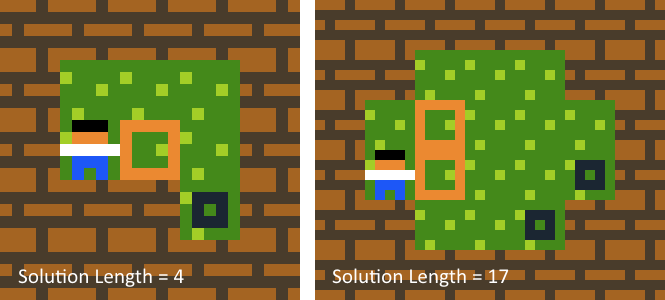
\includegraphics[width=0.45\textwidth]{Images/sokobanLenghtArea}
	    \label{Figure:sokobanLenghtArea}
	    \caption{Examples of two sokoban levels with different area and solution lengths}
	\end{figure}
	
	From the previous example we can conclude that the solution length depends on the level area. Instead of using the solution length as the metric we used the ratio between the solution length and the level area. A mapping function is used to convert that number to a value in the range of [0, 1]. We analyzed 40 hand crafted levels with different area from 5 different games. A histogram is plotted for the ratio between the solution length and the level area and shown in \figref{solutionLengthHistogram}.
	
	\begin{figure}
		\centering
		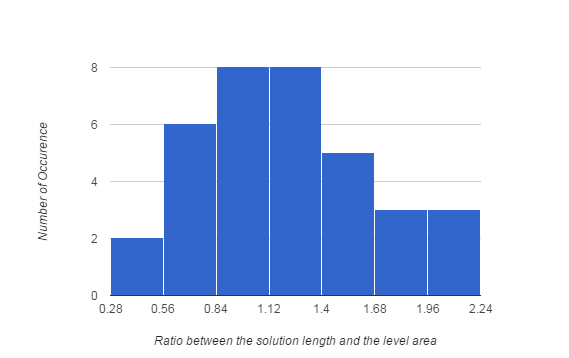
\includegraphics[width=0.45\textwidth]{Images/solutionLengthHistogram}
		\label{Figure:solutionLengthHistogram}
		\caption{Histogram for the ratio between the solution length and the level area}
	\end{figure}
	
	The histogram seems to follow a Normal Distribution with $\mu = 1.221$ and $\sigma = 0.461$. Based on that, the Solution Length Score is expressed by the following equation:
	\begin{center}$L_{score} = Normal(\dfrac{L}{A}, 1.221, 0.461)$\end{center}
	where $Normal(ratio, \mu, \sigma)$ is a normal distribution function, $L$ is the solution length, and $A$ is the level area.
	
	\item \emph{Object Number Score ($N_{score}$):} The Object Number Score is calculated by the following equation:
	\begin{center}$N_{score} = 0.4 * N_{rule} + 0.3 * N_{player} + 0.3 * N_{winning}$\end{center}
	where $N_{rule}$ is the Number of Rule Objects ratio, $N_{player}$ is the Number of Players value, and $N_{winning}$ is the Number of Winning Objects value.
	\begin{itemize}
		\item \emph{Number of Rule Objects ($N_{rule}$):} In a good designed level, most of the rule objects should appear in the level to ensure there is a possibility of applying every rule. The number of times the object should appear in the level must be greater than or equal his minimum number property from the Rule Analyzer. A ratio is calculated between the number of objects greater than their minimum number property and the total number of the rule objects.
		\begin{center}$N_{rule} = \dfrac{N_{min}}{N_{max}}$\end{center}
		where $N_{min}$ is the number of objects greater than their minimum number property and $N_{max}$ is the total number of the rule objects.
		\item \emph{Number of Players ($N_{player}$):} The game should have only one player. If any level have a different value, the score will be zero.
		\begin{center}
		$N_{player}= \begin{cases}
		               1 & \text{one player object exists}\\
		               0 & \text{otherwise}
		           \end{cases}$
		\end{center}
		\item \emph{Number of Winning Objects ($N_{winning}$):} The number of the winning objects should be equal, unless one of the winning objects have "Create" behavior. Based on the previous condition, the score is set to either one or zero.
		\begin{center}
			$N_{winning}= \begin{cases}
			               1 & \ N_{winnObj1} == N_{winObj2} \text{ and no Create behavior}\\
			               1 & \text{Create behavior exists}\\
			               0 & \text{otherwise}
			           \end{cases}$
		\end{center}
		where $N_{winObj1}$ is the number of the first winning object and $N_{winObj2}$ is the number of the second winning object.
	\end{itemize}
	
	\item \emph{Box Line Score ($B_{score}$):} It is similar to Taylor and Parberry\cite{sokobanLevelGenerationNew} metric to find the farthest state. This metric calculates the number of unrepeated moves found in the solution and divide it by the solution length. The following equation represents it:
	\begin{center}$B_{score} = \dfrac{L_{unique}}{L}$\end{center}
	where $L_{unique}$ is the number of unrepeated moves in the solution and $L$ is the solution length.
	
	\item \emph{Applied Rule Score ($R_{score}$):} Good level design involves applying game rules for a number of times to solve any level. The ratio between the number of applied rules to the solution length should be used for indicting good level design. Exaggerating in applying the rules results in boring level. Same can be said for the very low amount of applying. \figref{sokobanRuleScore} shows two levels from Sokoban with different solutions. The left level needs to apply Sokoban's rule for one time to solve the level, while the right needs to apply Sokoban's rule with every single step.
	
	\begin{figure}
		\centering
		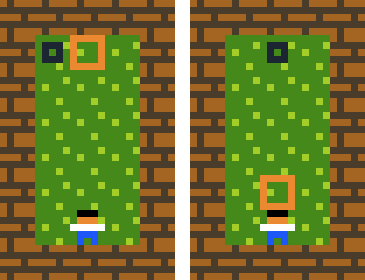
\includegraphics[width=0.45\textwidth]{Images/sokobanRuleScore}
		\label{Figure:sokobanRuleScore}
		\caption{Example for two boring levels from Sokoban}
	\end{figure}
	
	To find the best ratio between both, We analyzed 40 hand crafted levels from 5 different games. A histogram is plotted for the ratio between the number of applied rules and the solution length and shown in \figref{rulesSolutionLengthHistogram}.
	
	\begin{figure}
		\centering
		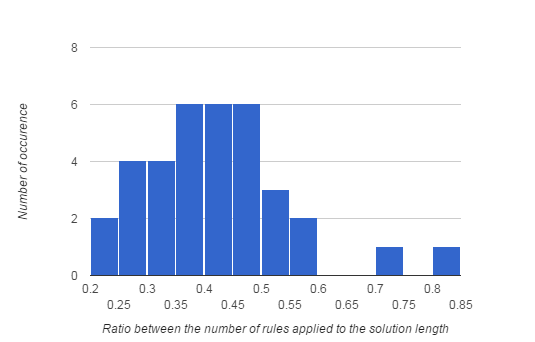
\includegraphics[width=0.45\textwidth]{Images/rulesSolutionLengthHistogram}
		\label{Figure:rulesSolutionLengthHistogram}
		\caption{Histogram for the number of rules applied to the solution length}
	\end{figure}
	
	The histogram seems to follow a Normal Distribution with $\mu = 0.417$ and $\sigma = 0.128$. Based on that the Applied Rule Score can be expressed by the following equation:
	\begin{center}$R_{score} = Normal(\dfrac{R_{applied} \pm R_{none}}{L}, 0.417, 0.128)$\end{center}
	where $Normal(ration, \mu, \sigma)$ is a normal distribution function, $R_{applied}$ is the number of applied rules, $R_{none}$ is the number of applied rules with no action associated, and $L$ is the solution length. The $R_{none}$ is used to decrease the normal distribution value according to amount of rules applied at the beginning of the game with no action associated to decrease them from happening.
	
	\item \emph{Exploration Score ($E_{score}$):} The increase in the number of explored states by the automated player means that the current level is not obvious to be solved directly by the automated player heuristics. This does not mean exploring huge space without finding a solution is better than exploring small number of states with a solution. The following equation express this idea:
	\begin{center}
	$E_{score}= \begin{cases}
	               0.75 + \dfrac{N_{explored}}{N_{max}} & \text{solution exists}\\
	               0.5 & \text{no solution and }N_{explored} = N_{max}\\
	               0 & \text{no solution and }N_{explored} < N_{max}
	           \end{cases}$
	\end{center}
	where $N_{explored}$ is the number of explored states and $N_{max}$ is the maximum number of states the automated player can explore.
\end{itemize}

\section{Results and Evaluation}

\section{Conclusion and Future Work}
This research presented a system to generate levels and rules for Puzzle Script. Also, it proposed several metrics to evaluate puzzle levels and games based on their solution sequence.\\\par

The proposed system generates levels regardless of the game rules. It uses two different techniques (Constructive and Genetic approach). The constructive approach resulted in 90\% playable levels which is enhanced in the genetic approach to reach 100\%, but it needs more time. Genetic approach uses GA with three different initialization methods (Random initialization, Constructive initialization, and Mixed initialization). Random initialization produces levels with different configuration from the constructive approach, but with low playability equals to 75\%.  The constructive approach produces levels with playability reaching 100\%, but with similar structure to the constructive approach. The mixed initialization is similar to constructive initialization in terms of playability but it expands the search space.\\\par

The generated levels are tested using human players\footnote{http://www.amidos-games.com/puzzlescript-pcg/} and a score is given for each level. Comparing the human scores with the system scores indicate a high correlation. This high correlation is a good indication that the proposed metrics can actually measure game playability and challenge. The correlation is higher in some games such as BlockFaker and Sokoban due to the high performance of the automated player in playing them.\\\par

This work is a first stone in general level and rule generation. There is a plenty to be done to expand and enhance it. As for future work, we aim to:
\begin{itemize}
	\item analyze the effect of each metric on the level generation.
	\item utilize the metrics to analyze the search space for level generation.
	\item test different techniques rather than plan GA to increase the level diversity like in Sorenson and Pasquier work\cite{genericLevelFramework}.
	\item improve the time and the quality of the automated player to decrease the generation time.
	\item generate levels with a specific difficulty.
\end{itemize}

\section{Acknowledgments}
I would like to express my deepest gratitude to Micheal Cook. His wok on ANGELINA was my main inspiration to start working on Procedural Content Generation. I would like to thank my supervisor Prof. Magda Fayek for all the support, guidance, and extreme patience she provides. Without her support this work would not have seen the light. Also Thanks to all my friends for the support and the huge help in collecting human feedback on the results.

\bibliographystyle{iccc}
\bibliography{iccc}

\end{document}